\documentclass[fleqn]{article}
\usepackage[utf8]{inputenc}
\usepackage{fullpage}
\usepackage[english]{babel}
\usepackage[pdftex]{graphicx}
\usepackage{float}
\usepackage{subcaption}
\usepackage{todonotes}
\usepackage[fleqn]{amsmath}
\usepackage{spverbatim}
\usepackage{longtable}
\usepackage{color, colortbl}
\newcommand{\HRule}{\rule{\linewidth}{0.5mm}}

\begin{document}

\begin{titlepage}

\begin{center}


% Upper part of the page

\includegraphics[width=0.5\textwidth]{epl-logo.png}\\[1cm]

\textsc{\LARGE catholic university of louvain-la-neuve}\\[1.5cm]

\textsc{\Large INGI2143 - Concurrent Systems}\\[0.5cm]


% Title
\HRule \\[0.4cm]
{ \huge \bfseries Report - Assignment 2}\\[0.4cm]

\HRule \\[1.5cm]

% Author

{\huge Alexandre \textsc{Hauet} \\[0.6cm] Florian \textsc{Thuin}}


\vfill

% Bottom of the page
{\large \today}

\end{center}

\end{titlepage}


\section{Introduction}

\todo[inline]{Ajouter l'explication de chaque fichier + observations/problèmes }


\section{Minimization of ELECTIONSERVICE vs multiple minimizations}

\begin{tabular}{l|p{0.25\linewidth}|l|l|l}
	Process & Alphabet & Number of states & Minimiz. time & Cum miniz. time \\
    \hline
    ELECTIONSERVICE(3) & [0..2].{close, open} & 740 & 52min & 52min \\
    ABSTRACT0(3) & [0..2].{{close, open}, rcvclaim[0..2], rcvtoken, sndclaim[0..2], sndtoken} & 5652 & 501ms & 501ms \\
    ABSTRACT1(3) & [0..2].{{close, open}, rcvclaim[0..2], {rcvtoken, sndtoken}} & 4826 & 550ms & 1051ms \\
    ABSTRACT2(3) & [0..2].{close, open, rcvtoken, sndtoken} & 2192 & 547ms & 1598ms \\
    ABSTRACT3(3) & [0..2].{close, open, sndtoken} & 1793 & 55ms & 1653ms \\
    ABSTRACT4(3) & [0..2].{close, open} & 740 & 31995ms & 33648ms \\
\end{tabular}


\newpage
\section{Property OPENCLOSE}

\begin{figure}[!h]
  \centering
    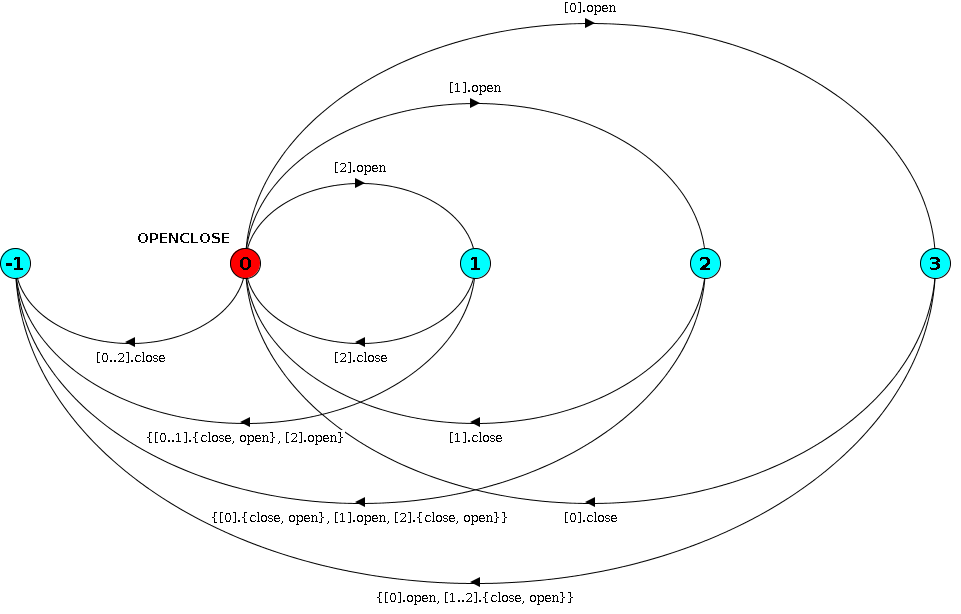
\includegraphics[width=\textwidth]{openclose_lts.png}
    \caption{Picture of the LTS of the property openclose}
\end{figure}


\section{Violation trace for OPENCLOSE on ELECTIONRING(3)}

\begin{figure}[h!]
\begin{equation*}
\begin{split}
	0.sndclaim.0 \rightarrow 1.rcvclaim.0 \rightarrow 0.sndclaim.0 \rightarrow 1.sndclaim.0 \rightarrow 1.rcvclaim.0 \rightarrow \\ 2.rcvclaim.0 \rightarrow 1.sndclaim.0 \rightarrow 2.sndclaim.0 \rightarrow 0.rcvclaim.0 \rightarrow 0.sndtoken \rightarrow \\
    1.rcvtoken \rightarrow \textcolor{red}{1.open} \rightarrow 2.rcvclaim.0 \rightarrow 2.sndclaim.0 \rightarrow 0.rcvclaim.0 \rightarrow \textcolor{red}{0.open}
\end{split}
\end{equation*}
\caption{The violation trace for OPENCLOSE on ELECTIONRING(3)}
\end{figure}

We can see with this trace that two nodes (1 and 0) want to access to the resource at the same time. It's a violation of the propety because the property define that a node can't access to the resource before an other node close it.


\newpage
\section{CRASHRING LTS}

\begin{figure}[!h]
  \centering
    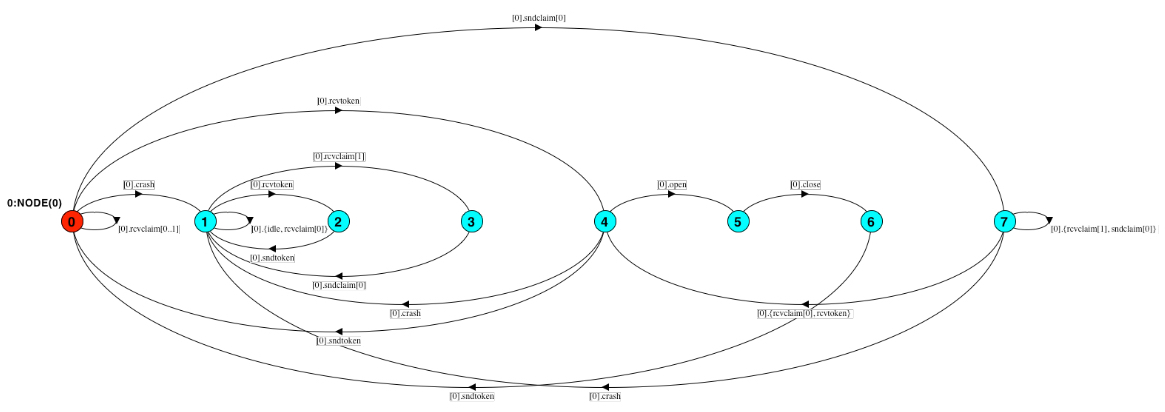
\includegraphics[width=\textwidth]{crashring.png}
    \caption{Picture of the LTS of a node in CRASHRING(2)}
\end{figure}


When a node crash, it realize the action ''crash'' to go in the state NODE\_CRASHED.

\section{ALLFAIR property}

Here is the violation trace for ALLFAIR on ELECTIONRING(3) without fair choice :
\begin{figure}[!h]
\begin{equation*}
\begin{aligned}
    0.sndclaim.0 \rightarrow 1.rcvclaim.0 \rightarrow 0.sndclaim.0 \rightarrow 1.sndclaim.0 \rightarrow 1.rcvclaim.0 \rightarrow 0.sndclaim.0 \rightarrow 2.rcvclaim.0 \rightarrow \\
    1.sndclaim.0 \rightarrow 1.rcvclaim.0 \rightarrow 2.sndclaim.0 \rightarrow 0.rcvclaim.0 \rightarrow 0.sndtoken \rightarrow 2.rcvclaim.0 \rightarrow 1.sndclaim.0 \rightarrow \\
    1.rcvtoken \rightarrow 0.sndclaim.0 \rightarrow 2.sndclaim.0 \rightarrow 0.rcvclaim.0 \rightarrow 2.rcvclaim.0 \rightarrow 1.sndtoken \rightarrow 1.rcvclaim.0 \rightarrow \\
    0.sndtoken \rightarrow 2.sndclaim.0 \rightarrow 2.rcvtoken \rightarrow 1.sndclaim.0 \rightarrow 1.rcvtoken \rightarrow 0.sndclaim.0 \rightarrow 0.rcvclaim.0 \rightarrow \\
    2.sndtoken \rightarrow 2.rcvclaim.0 \rightarrow 1.sndtoken \rightarrow 1.rcvclaim.0 \rightarrow 0.sndtoken \rightarrow 0.rcvtoken \rightarrow 2.sndclaim.0 \rightarrow  \\
    2.rcvtoken \rightarrow 1.sndclaim.0 \rightarrow 1.rcvtoken \rightarrow 0.sndtoken \rightarrow 0.rcvclaim.0 \rightarrow 2.sndtoken \rightarrow 0.rcvtoken \rightarrow    \\
    2.rcvclaim.0 \rightarrow 1.sndtoken \rightarrow 1.rcvtoken \rightarrow 0.sndtoken \rightarrow 2.sndclaim.0 \rightarrow 2.rcvtoken \rightarrow 1.sndtoken \rightarrow   \\
    1.rcvtoken \rightarrow 0.sndclaim.0 \rightarrow 0.rcvclaim.0 \rightarrow 2.sndtoken \rightarrow 2.rcvtoken \rightarrow 1.sndtoken \rightarrow 1.rcvclaim.0 \rightarrow  \\
    0.sndtoken \rightarrow 0.rcvtoken \rightarrow 2.sndtoken \rightarrow 2.rcvtoken \rightarrow 1.sndclaim.0 \rightarrow 1.rcvtoken \rightarrow 0.sndtoken \rightarrow     \\
    0.rcvtoken \rightarrow 2.sndtoken \rightarrow 2.rcvclaim.0 \rightarrow 1.sndtoken \rightarrow 1.rcvtoken \rightarrow 0.sndtoken \rightarrow 0.rcvtoken \rightarrow \\
    2.sndclaim.0 \rightarrow 2.rcvtoken \rightarrow 1.sndtoken \rightarrow 1.rcvtoken \rightarrow 0.sndtoken \rightarrow 0.rcvclaim.0 \rightarrow 2.sndtoken \rightarrow \\
    0.rcvtoken \rightarrow 2.sndclaim.2 \rightarrow 2.rcvtoken \rightarrow 1.sndtoken \rightarrow 1.rcvtoken \rightarrow 0.sndtoken \\
\end{aligned}
\end{equation*}
As this trace isn't really readable, the cycle in terminal set is :
\begin{equation*}
    \textcolor{red}{0.rcvclaim.2 \rightarrow 2.sndtoken \rightarrow 0.rcvtoken \rightarrow 2.sndclaim.2 \rightarrow 2.rcvtoken \rightarrow 1.sndtoken \rightarrow 1.rcvtoken \rightarrow 0.sndtoken}
\end{equation*}
\caption{The violation trace for ALLFAIR on CRASHRING(3)}
\end{figure}
We can explain this result : if the node is always in the election protocol (so never in the \textit{access resources} mode), there isn't any \verb#open# transition. However, it is only possible if there isn't a fair choice between the transition otherwise we would indefintely often access resources and the property ALLFAIR would be respected.


\section{MUTEX violation with increasing number of nodes}

We will not show the N=1 because the property isn't violated. \newline

Without Partial Order Reduction :

\bigskip
\begin{tabular}{l|l|l|l|l}
    N & Number of states & Number of transitions & Time & Length of violation trace \\
    \hline
    2 & 77               & 141                   & 0ms  & 13 \\
    3 & 858              & 2141                  & 1ms  & 17 \\
    4 & 9226             & 29467                 & 17ms & 21 \\
    5 & 117339           & 440519                & 195ms & 25 \\
    6 & 1842823          & 787101009               & 8575ms & 29 \\
\end{tabular}
\bigskip

With Partial Order Reduction :

\bigskip
\begin{tabular}{l|l|l|l|l}
    N & Number of states & Number of transitions & Time & Length of violation trace \\
    \hline
    2 & 74               & 131                   & 8ms   & 13 \\
    3 & 789              & 1753                  & 6ms   & 17 \\
    4 & 8135             & 20496                 & 39ms  & 21 \\
    5 & 96928            & 255807                & 272ms & 25 \\
    6 & 1387005          & 3737714               & 5599ms & 29 \\
\end{tabular}


\section{Checking MUTEX using Supertrace on ELECTIONRING(N)}
\begin{tabular}{l|p{0.25\linewidth}|l|l|l|l}
	N & Number of states & transitions & time & length of violation trace\\
    \hline
    1 & 6   &   7       &   0ms    &   0  \\
    2 & 27  & 49 & 0ms & 49 \\
    3 & 66  & 128 & 0ms & 128 \\
    4 & 123 & 248 & 0ms & 248\\
    5 & 198 & 409 & 1ms & 409\\
    6 & 271 & 597 & 1ms & 496\\
\end{tabular}


\section{Checking MUTEX using different Supertrace parameters}
We highlighted the results : red is when the violation of MUTEX isn't detected ; green is where the value is a minimum. 

\begin{longtable}{l|l|l|l|l|l}
HashTable size (Kb) & Search depth & Number of states & Transitions & Time & Length of violation \\
\hline
\rowcolor{red!40}1000 & 20 & 2179 & 9457 & 11ms & 0 \\
\rowcolor{red!40}20000 & 20 & 2179 & 9457 & 8ms & 0 \\
\rowcolor{red!40}40000 & 20 & 2179 & 9457 & 7ms & 0 \\
\rowcolor{red!40}60000 & 20 & 2179 & 9457 & 7ms & 0 \\
\rowcolor{red!40}80000 & 20 & 2179 & 9457 & 5ms & 0 \\
\rowcolor{red!40}100000 & 20 & 2179 & 9457 & 5ms & 0 \\
\rowcolor{red!40}20000 & 50 & 8776 & 35035 & 16ms & 0 \\
\rowcolor{red!40}20000 & 75 & 29168 & 105429 & 42ms & 0 \\
\rowcolor{red!40}20000 & 80 & 81363 & 305813 & 126ms & 0 \\
\rowcolor{red!40}1000 & 91 & 42277 & 148390 & 57ms & 0 \\
\rowcolor{red!40}1000 & 92 & 59624 & 217178 & 85ms & 0 \\
1000 & 93 & 69577 & 255080 & 100ms & 50 \\
\rowcolor{red!40}1000 & 94 & 72925 & 263255 & 103ms & 0 \\
1000 & 95 & 91889 & 332664 & 112ms & \cellcolor{green!40}45 \\
100000 & 95 & 93801 & 339557 & 152ms & \cellcolor{green!40}45 \\
\rowcolor{red!40}1000 & 96 & 71452 & 260285 & 95ms & 0 \\
1000 & 97 & 94180 & 338071 & 141ms & 55 \\
20000 & 97 & 91236 & 327673 & 114ms & 56 \\
1000 & 98 & 63359 & 230983 & 93ms & 47 \\
1000 & 99 & 67496 & 239471 & 85ms & 51 \\
20000 & 100 & 63539 & 223387 & 95ms & 51 \\
500 & 150 & 1204 & 3666 & 4ms & 75 \\
1000 & 150 & 1204 & 3666 & 2ms & 77 \\
20000 & 150 & 1204 & 3666 & 2ms & 75 \\
1000 & 200 & \cellcolor{green!40}139 & \cellcolor{green!40}280 & 1ms & 96 \\
1000 & 300 & 150 & 308 & 0ms & 148 \\
1000 & 400 & 246 & 527 & 0ms & 193 \\
1000 & 500 & 198 & 409 & 1ms & 198 \\
20000 & 500 & 198 & 409 & 1ms & 198 \\
40000 & 500 & 198 & 409 & 1ms & 198 \\
60000 & 500 & 198 & 409 & 1ms & 198 \\
80000 & 500 & 198 & 409 & 1ms & 198 \\
100000 & 500 & 198 & 409 & 0ms & 198 \\
1000 & 1000 & 198 & 409 & 0ms & 198 \\
20000 & 1000 & 198 & 409 & 0ms & 198 \\
40000 & 1000 & 198 & 409 & 0ms & 198 \\
60000 & 1000 & 198 & 409 & 0ms & 198 \\
80000 & 1000 & 198 & 409 & 0ms & 198 \\
100000 & 1000 & 198 & 409 & 0ms & 198 \\
1000 & 1500 & 198 & 409 & 0ms & 198 \\
20000 & 1500 & 198 & 409 & 0ms & 198 \\
40000 & 1500 & 198 & 409 & 0ms & 198 \\
60000 & 1500 & 198 & 409 & 0ms & 198 \\
80000 & 1500 & 198 & 409 & 1ms & 198 \\
100000 & 1500 & 198 & 409 & 1ms & 198 \\
1000 & 2000 & 198 & 409 & 0ms & 198 \\
20000 & 2000 & 198 & 409 & 0ms & 198 \\
40000 & 2000 & 198 & 409 & 0ms & 198 \\
60000 & 2000 & 198 & 409 & 0ms & 198 \\
80000 & 2000 & 198 & 409 & 0ms & 198 \\
100000 & 2000 & 198 & 409 & 0ms & 198 \\
\end{longtable}

As we can see among the results in the table, the values that lead to the shortest trace are the ones with a search depth of 95. The length of the violation trace increases as the search depth increases but its maximum value (198) is reached when the search depth is greater than 500. \newline

We can also see that the amount of states and transitions decreases as the search depth or the HashTable size increases. \newline


\section{Conclusion}
\input{conclusion.tex}
\end{document}
